\documentclass{article}
\usepackage[utf8]{inputenc}
\usepackage{graphicx}

\title{Autonomous Agents \\ Assignment 1 \\ Group 2}
\author{Louis Smit (10678697) \\ Jerome Cremers (10470425) \\
Hubert Szostek (10656804) \\ Lex Utama (10660356)}
\date{September 2013}

\begin{document}

\maketitle

\section{Introduction}
In this assignment several single agent planning methods are implemented on a predator-prey game, as decribed in the assignment. The basic environment is an 11x11 grid (\ref{Grid}). The grid is
toroidal: the north side of the grid is attached to the south side, and the east side is attached to the west side. The predator and the prey can be anywhere on this grid, though they cannot be on the same square. The starting position of the prey is (5,5) and that of the predator (0,0).\\
Obviously, the goal for the predator is to catch the prey. This happens when the predator stands next to the prey, and moves in the direction of the prey. When the prey is captured, the episode ends, and the game is reverted to the starting position.

\begin{figure}[hb]
  \centering
  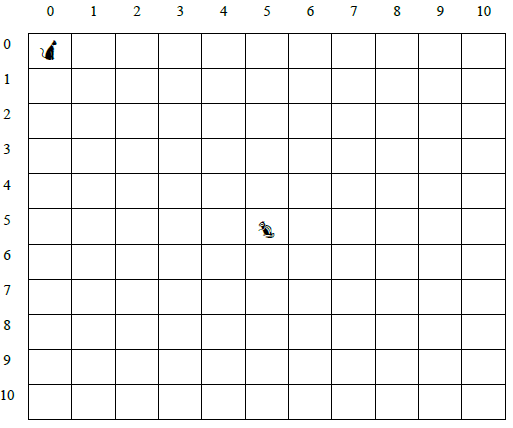
\includegraphics[width=3.3in]{Grid_world}
  \caption[Figure 1]
   {The predator-prey environment: a 11x11 toroidal grid, in the starting position. The predator is depicted by the cat, and the prey by the squirrel.}
   \label{Grid}
\end{figure}


\section{Implementation}
The game is implemented in Java. Eclipse was used as a code editor and compiler. \\
Classes\\
State space representation\\
Policy Evalutation\\
Value iteration\\
Tests\\

\section{Results}

\section{Conclusion}

\end{document}
